\section{Setting the landscape on entrepreneurship and private investment}

\begin{figure}[h]
    \centering
    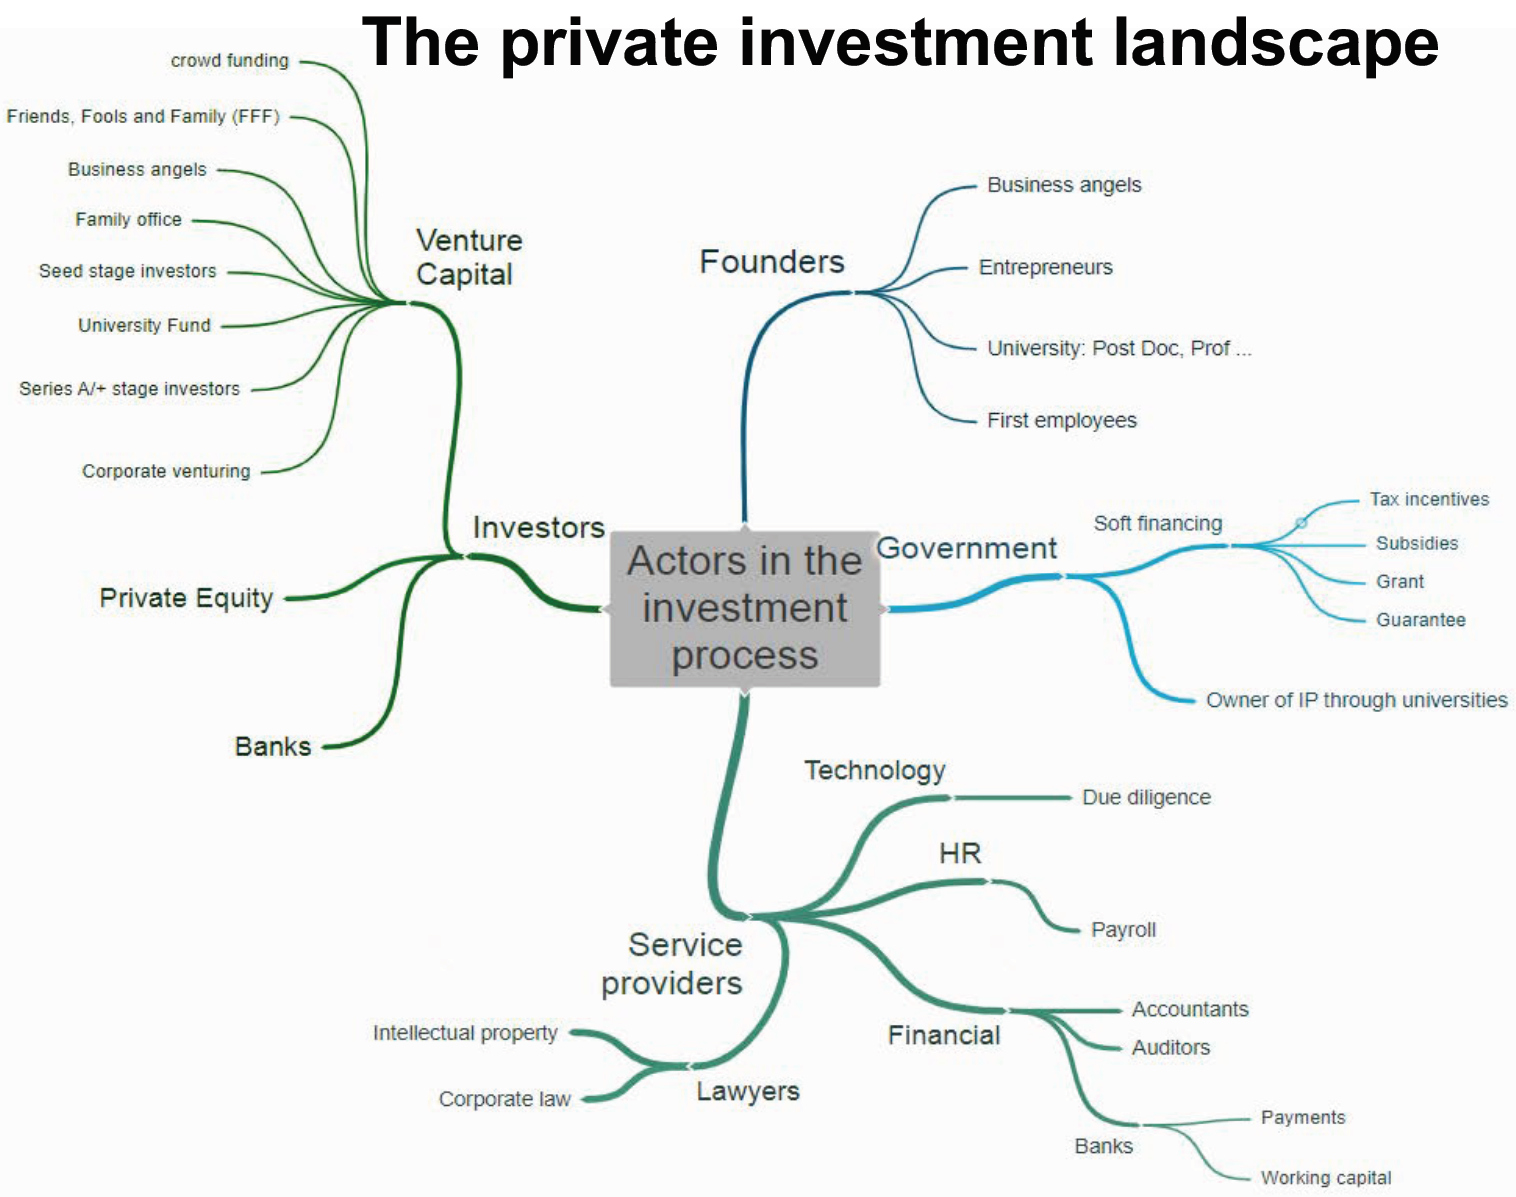
\includegraphics[width=0.8\textwidth]{Pictures/private_investment_landscape.png}
    \caption{Private investment landscape}
    \label{private_investment_landscape}
\end{figure}


\paragraph{Difference between Private Equity and Venture Capital}

\begin{definition}[Private equity]
    \begin{itemize}
        \item Financing mainly used to buy mature well-established companies
        \item and get full control (100\% of company)
        \item Always a combination of debt and equity (shares)
        \item Calue created through streamlining of operations, cost cutting, consolidation\dots
        \item Strong fucus on cash flow to pay of debt, companies are highly leveraged (much debt relative to equity)
        \item Leverage increases risk profile but also potential returns.
        \item Large deal sizes (hundreds of millions)
    \end{itemize}
\end{definition}

\begin{definition}[Venture capital]
    \begin{itemize}
        \item Financing mainly given to startup companies and small businesses
        \item Value created through growth
        \item Growth expected from innovation, disruptive technology, new product, business plan
        \item Very high risk profile, no cash flow but cash burn (that is where the money is used for)
        \item Company can only finance through equity, often risk profile is too high to get debt financing
        \item Smaller deal sizes (millions)
        \item No full control (50\% or less)
    \end{itemize}
\end{definition}

\begin{definition}[Asset and leverage]
    \begin{align*}
        \text{Asset} = \text{Debt} + \text{Equity}
        \hspace{10pt} , \hspace{10pt}
        \text{Leverage} = \frac{\text{Asset}}{\text{Equity}} = \frac{\text{Debt}}{\text{Equity}} + 1
    \end{align*}
\end{definition}

Most new businesses do not survive the first five years.
Investors want to manage their risk with preference shares and by gaining as much
control as possible on the company, through shareholder agreements, voting rights,
board membership, anti-dilution clauses\dots

\paragraph{Liquidation preferences}
\begin{itemize}
    \item Much VCs invest using so-called 'preference shares' instead of common shares.
    \item In the event of the failure of the company, preferred shareholders may receive payment from liquidation before common shareholders.
    \item When the company is sold (at the so-called exit), preferred shareholders may receive
        payment (sometimes with a guaranteed ROI) in full before the common shareholders.
\end{itemize}

The pay-off is highly skewed, many loosers and a few big winners.
Investors must be detached from individual companies and look at the whole
portfolio. This is not aligned with the Entrepreneurs' viewpoint.

\vspace{1\baselineskip}

Risk and return are like Yin and Yang

\begin{figure}[h]
    \centering
    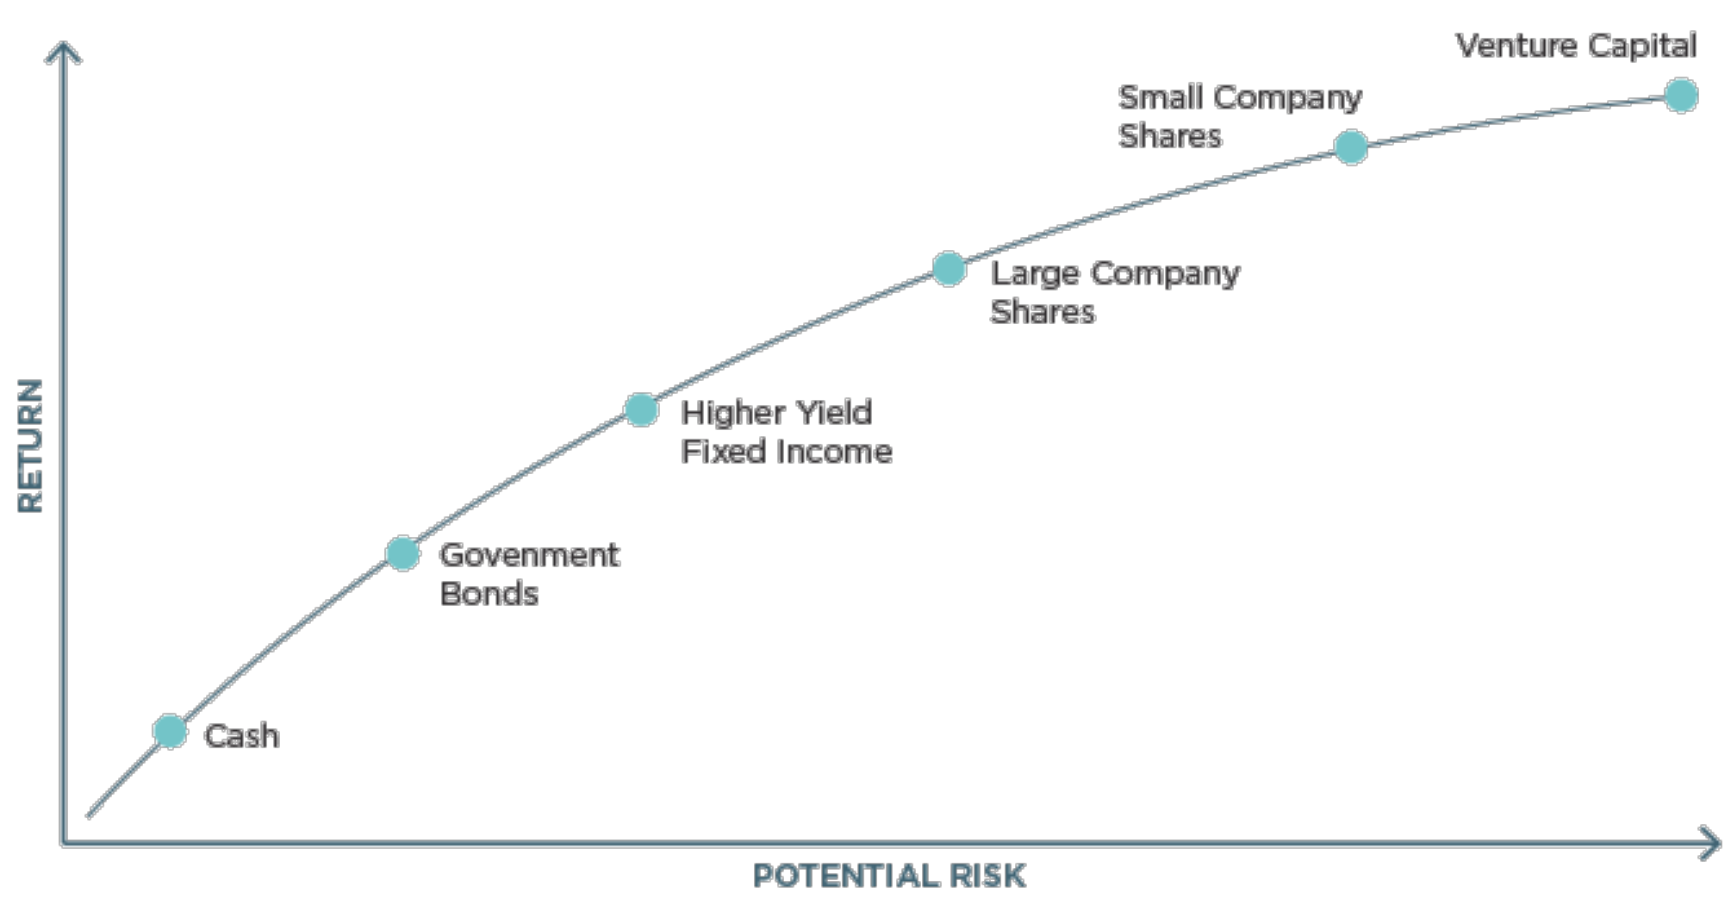
\includegraphics[width=0.5\textwidth]{Pictures/potential_risk_return_graph.png}
\end{figure}

\paragraph{Perceived vs. actual risk}
Two kinds of bias were identified: (a) a tendency to overestimate small frequencies
and underestimate larger ones; and (b) a tendency to exaggerate the frequency of
some specific causes and to underestimate the frequency of other, at any given level
of objective frequency.

\paragraph{Prospect Theory: Kahnman and Tversky}
"Losses loom larger than gains." Individuals assess losses and gains in an
asymmetric way e.g. for some people, the pain from losing 1000 USD could
only be compensated by the pleasure of earning 2000 USD.

\paragraph{Viewpoints of Investors and Entrepreneurs} \

\begin{figure}[h]
    \centering
    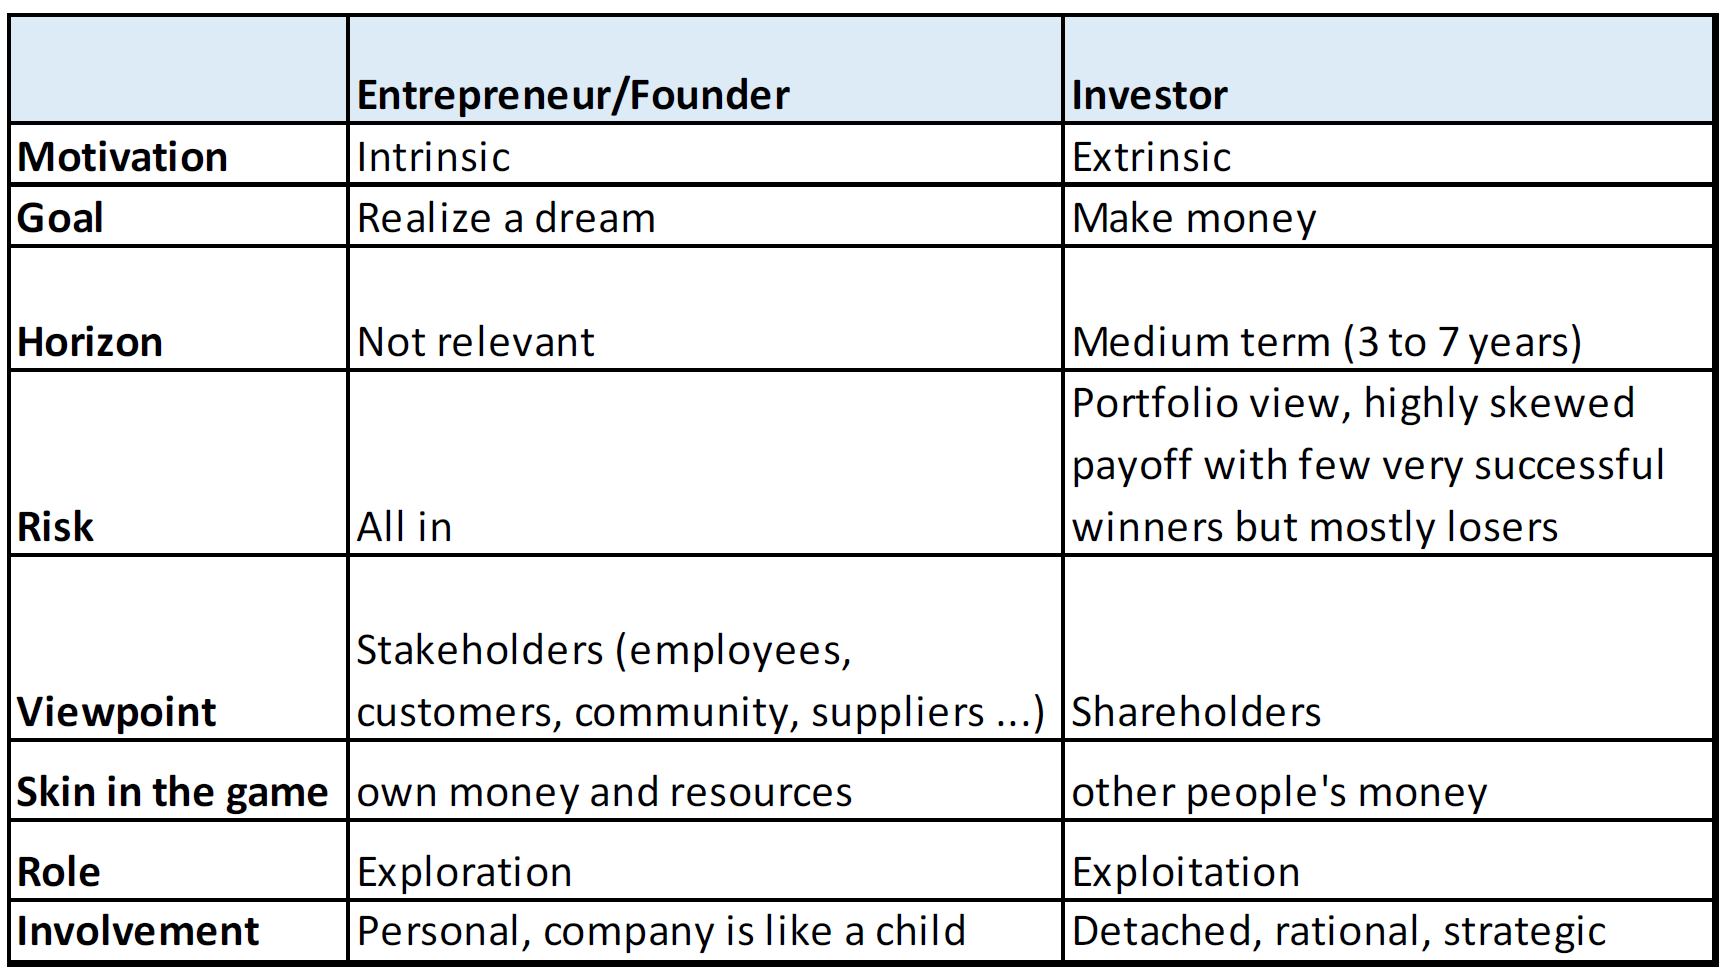
\includegraphics[width=0.5\textwidth]{Pictures/viewpoints_entrepreneurs_investors.png}
\end{figure}

\paragraph{Challenges of exploration}
According to Herbert Simon exploration requires:
\begin{itemize}
    \item tolerance of ambiguity/uncharted territory
    \item patience: learning-by-doing, accumulation of knowledge, trial-and-error
    \item luck / serendipity
    \item persistence / diligence
    \item 'intuition': use of smart heuristics
\end{itemize}
It is a high risk endeavor, where the payoff is almost impossible to estimate.

\paragraph{Exploitation}
Exploitation is tempting from a short-term risk/return perspective, but there are
serious caveats on the long run.

\begin{figure}[h]
    \centering
    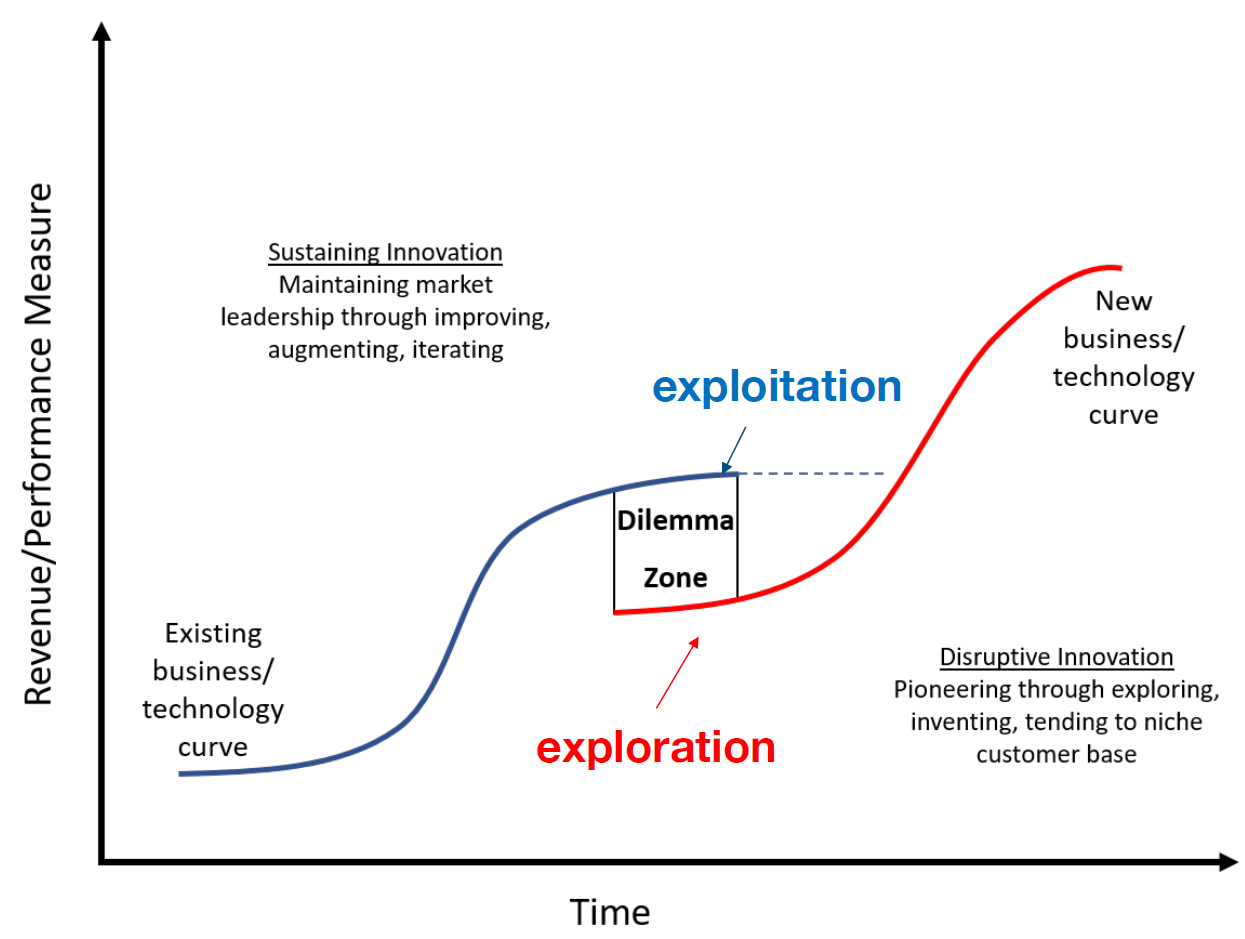
\includegraphics[width=0.5\textwidth]{Pictures/exploration_exploitation_curve.png}
\end{figure}

Disruptive innovations are initially too small to meet the ROI-targets of large
established firms. However, they steadily work their way up eventually
capitalizing on a crucial first mover advantage against large, less nimble,
market leaders.

\paragraph{Important Terms}
\begin{itemize}
    \item Regression to the mean
    \item Narrow Framing
\end{itemize}

\paragraph{How to deal with biases?}
\begin{itemize}
    \item \underline{Heuristics}: When predictability is poor, inconsistency,
        based on unnoticed stimuli, is destructive of any predictive validity.
        Be consistent by using investment criteria, simple formular, recipies
        or rules of thumb.
    \item \underline{Example, consider an outside view}: Prior to the use of any
        inside information, try to predict a totally independent base rate e.g.
        "how many start-ups in this field survive the first three years?"
        Use this as your anchor and adjust this base rate according to information
        obtained during the due diligence.
    \item \underline{Decorrelate error}: Ask people's opinion indepentently of each
        other, wisdom of crowds vs. group think, practice "constructive confrontation",
        avoid "cozy unanimity"
    \item \underline{Sunk Cost}: Be aware of the difficulty to take a loss. A new
        manager does not carry the same mental accounts and is therefore more
        able to ignore the sunk of past investments.
    \item \underline{Validity of intuition}: Intuition cannot be trusted in the
        absence of stable regularities in the environment and in the absence of
        prolonged practice and learning.
\end{itemize}

\paragraph{Closing a deal}
Only a fraction (0.5-2\%) of considered deals get closed.

\begin{figure}[h]
    \centering
    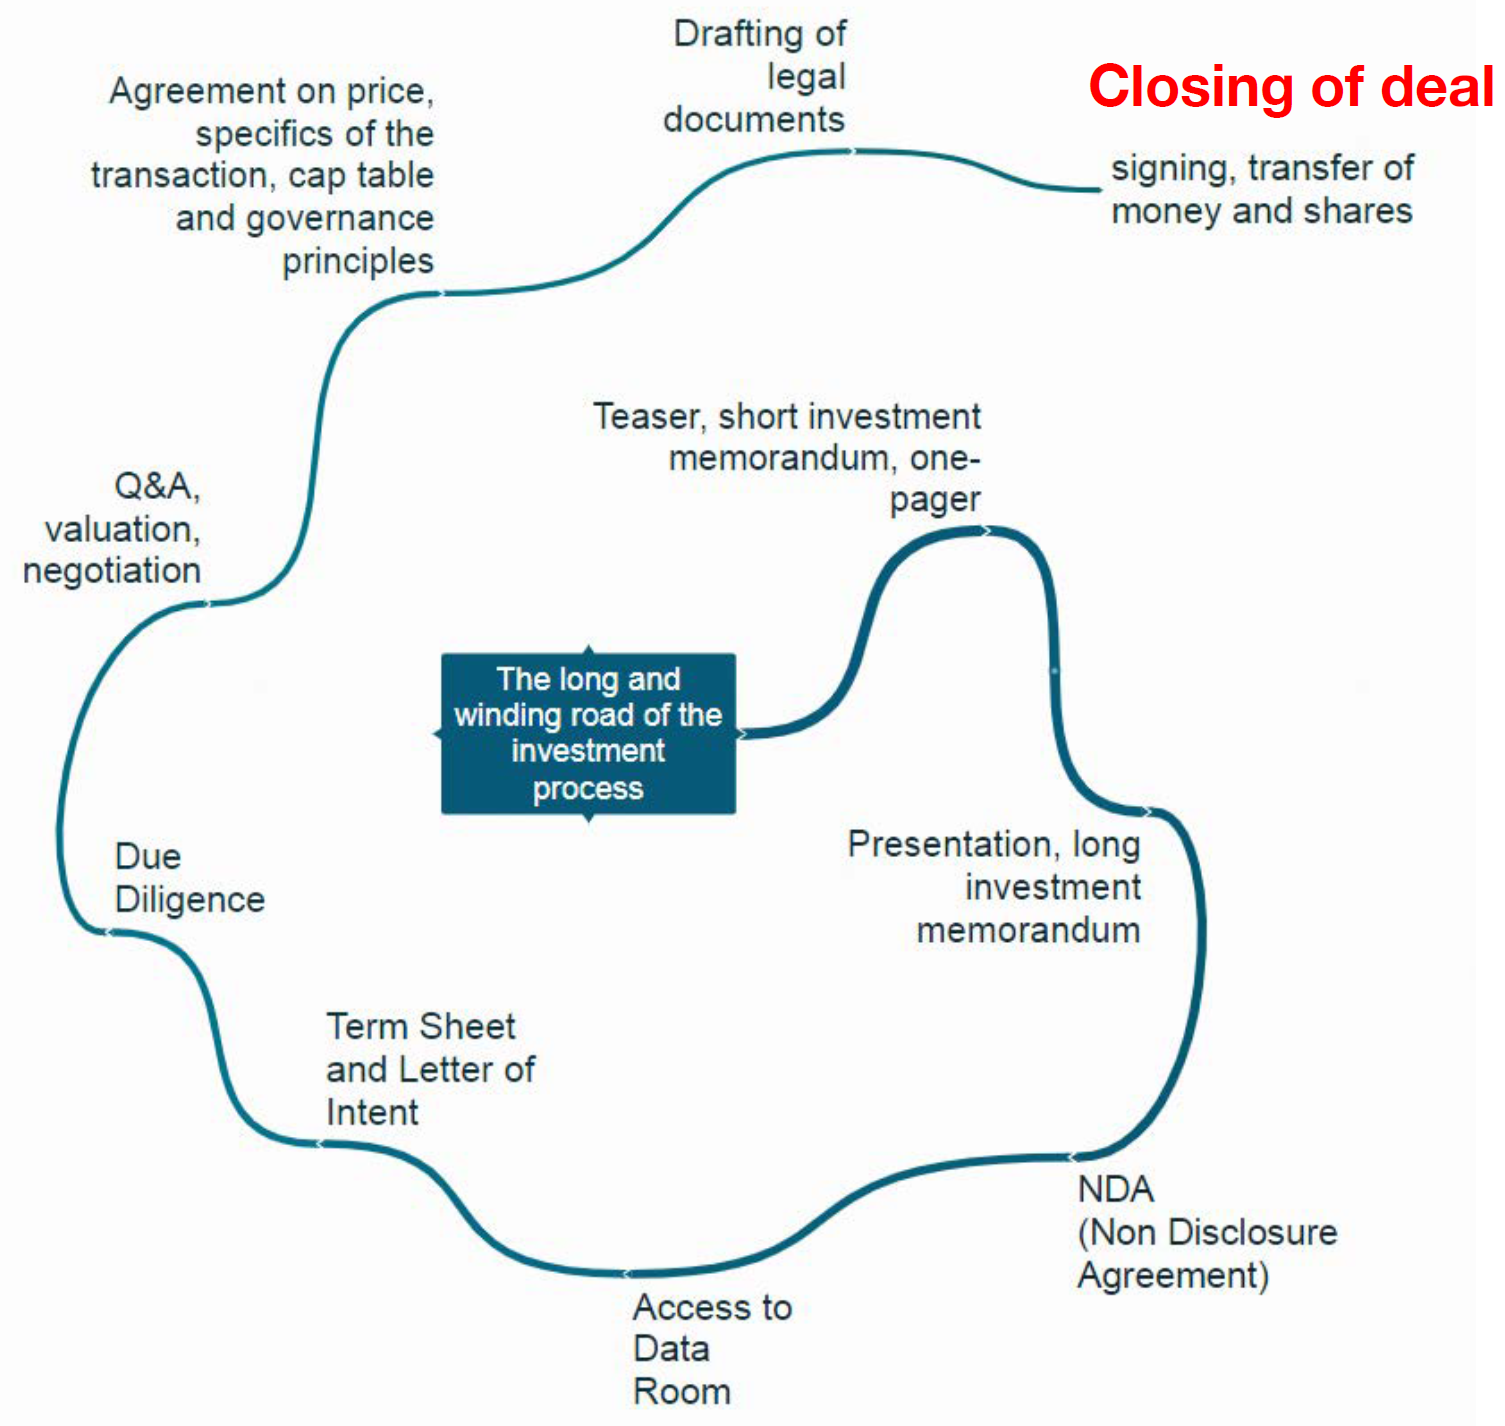
\includegraphics[width=0.45\textwidth]{Pictures/closing_Deal.png}
\end{figure}

\paragraph{Pitch Deck}
\begin{itemize}
    \item Sales pipeline, proven market interest, test by the market\dots
    \item Growth strategy: sales, product development, scalability, BOM
    \item Investment: Use of proceeds
    \item Current cap table
    \item Exit options for investor
\end{itemize}

\begin{figure}[h]
    \centering
    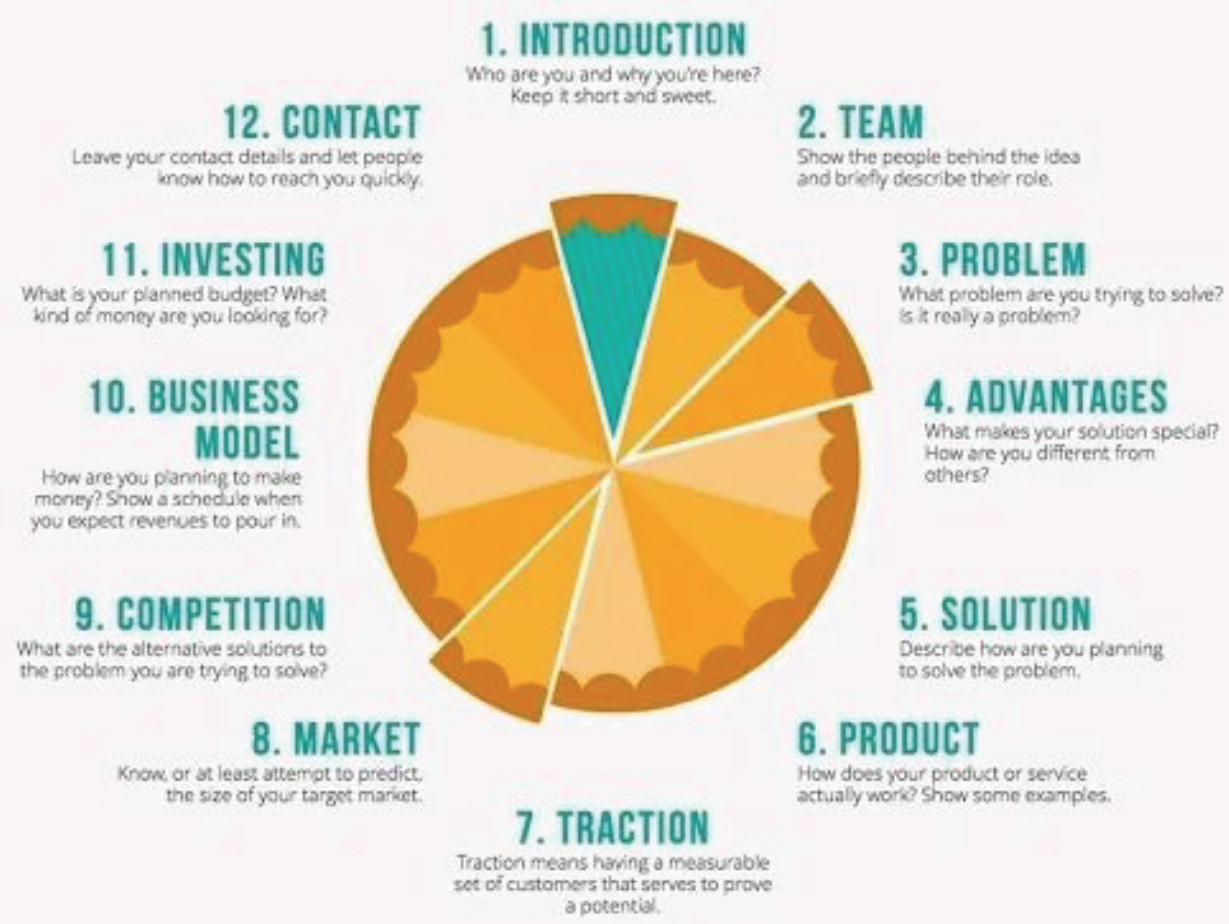
\includegraphics[width=0.8\textwidth]{Pictures/12_slides_of_a_pitch_deck.png}
    \caption{Pitch Deck}
\end{figure}

\paragraph{Get to know each other}
Possible Questions:
\begin{itemize}
    \item Team:
        \begin{itemize}
            \item Does your company culture and values math with us?
            \item Are there complementary skills in your core team?
            \item Can you give references for your key employees? 
        \end{itemize}
    \item Technology:
        \begin{itemize}
            \item What makes your technology unique?
            \item How is the Intellectual Property proteted?
        \end{itemize}
    \item Product:
        \begin{itemize}
            \item Is it developed beyond the design phase?
            \item How does it scale?
            \item How does your bill of materials (BOM) change with production volumes?
        \end{itemize}
    \item Market:
        \begin{itemize}
            \item Do you understand the market?
            \item How do you plan to access the market?
            \item How big is the market?
            \item What market share are you targeting?
        \end{itemize}
    \item Sales:
        \begin{itemize}
            \item Describe your customer. Can you give references?
            \item What are their problems and how do your provide solutions?
            \item How are your sales distributed over the customers?
            \item What kind of sales process do you have? Direct vs distributed sales?
                Do you have salespeople with experience, a trustworthy pipeline, good lead customers?
            \item Do you have a ROI model for your client, or do you deliver a nice-to-have product?
        \end{itemize}
    \item Economics:
        \begin{itemize}
            \item Do you understand the big trends?
            \item Does your product serve a long-term goal, service a need?
            \item How does your product fit the big changing trands?
        \end{itemize}
    \item Financials:
        \begin{itemize}
            \item Do you have a storng and robust business plan?
            \item Do you understand you future cash flow?
            \item Do you understand the risks?
            \item What are the sensitivities? Worst case scenario?
            \item Do you have a fallback/plan-B?
        \end{itemize}
\end{itemize}


Also ask the investors what their interests and terms are.

\paragraph{NDA - Non-Disclosure Agreement}

If the introduction round is finished successfully a Non-Disclosure Agreement (NDA)
is signed between the investor and the founders. This is a legal contract that outlines
the use of confidential material, knowledge and information that the parties wish
to exchange. After the NDA is signed by both parties, access is given to the data
room.

\paragraph{Term sheet / Letter of Intent}
After a first check of the data room, the investors will produce a term sheet or
LOI, this outlines an agreement that two or more parties exept to make. Term
sheet and LOI are very similar in content, but TS is structured as a list, often
in a table format, whereas LOI is in the form of a letter. Written before the
execution of a formal and binding contract, most of the listed agreements are
not legally binding.
Topics are:
\begin{itemize}
    \item Valuation of the company
    \item Amount of investment
    \item Use of proceeds
    \item Cap table
    \item Share preferences
    \item Governance (Board composition and chair)
    \item Investor commitment
    \item Management commitment
    \item Exit (right of first refusal)
    \item Description of the Due Diligence process (time, topics,\dots)
    \item Exclusivity
\end{itemize}

\paragraph{Exclusivity}
Legal binding clause of the LOI or TS. Caveat: Transfers a lot of control to
the investor, he/she will be the only party taking the next step in the process,
he/she can take advantage of the 'sunk cost effect', often exclusivity periods
are extended. When giving exclusivity, time is on the side of the investor.
The investor can put you under pressure, test your tenacity and patience, try
to decrease the valuation of the company. When you give exclusivity, you cancle
out any competition for the investor, this will make him/her dominant.

\paragraph{Due diligence}
After the Term Sheet and/or the Letter of Intent are signed, the Due Diligence
process is started. This is supposed to take only up to six weeks, in reality,
it will turn out to be many months. Now, the external advisors enter the arena.
\begin{itemize}
    \item \underline{Business lawyers}: will examine all the contracts in the data room.
    \item \underline{IP lawyers}: will study the strengths of the patents of the company
        and the 'freedom to operate'
    \item \underline{External auditor}: will validate the accounting, finance statements,
        balance sheet, taxes
    \item \underline{Technological consultant}: may analyze the product development
        and the strength and relevance of the technology with respect to other solutions.
\end{itemize}
Investors themselves will:
\begin{itemize}
    \item Do reference checks of clients, founders, key personal.
    \item Analyze the commercial viability of the product and the sales process
        and tools.
    \item Study the quality of the sales pipeline.
    \item Based on that will make their own forecast of future sales.
    \item And a forecast of future cashflows.
\end{itemize} 
Based on the results of the due diligence, the investors will challenge the
business plan. This will allow them to:
\begin{itemize}
    \item Create base-case and worst-case scenarios of cash burn
    \item Check the investment amount and the use of proceeds with respect to these
        scenarios, are the founders asking too much, too little?
    \item Assess the risk of their investment.
    \item Set goals, milestones for the Management
    \item Find the gaps, see where the company needs further support
    \item Check, whether some of these gaps are a no-go
    \item Possibly discuss releasing the invested amount in tranches, each time
        when a certain milestone is reached.
    \item Make their own valuation of the company.
\end{itemize}
